\PassOptionsToPackage{unicode=true}{hyperref} % options for packages loaded elsewhere
\PassOptionsToPackage{hyphens}{url}
%
\documentclass[]{article}
\usepackage{lmodern}
\usepackage{amssymb,amsmath}
\usepackage{ifxetex,ifluatex}
\usepackage{fixltx2e} % provides \textsubscript
\ifnum 0\ifxetex 1\fi\ifluatex 1\fi=0 % if pdftex
  \usepackage[T1]{fontenc}
  \usepackage[utf8]{inputenc}
  \usepackage{textcomp} % provides euro and other symbols
\else % if luatex or xelatex
  \usepackage{unicode-math}
  \defaultfontfeatures{Ligatures=TeX,Scale=MatchLowercase}
\fi
% use upquote if available, for straight quotes in verbatim environments
\IfFileExists{upquote.sty}{\usepackage{upquote}}{}
% use microtype if available
\IfFileExists{microtype.sty}{%
\usepackage[]{microtype}
\UseMicrotypeSet[protrusion]{basicmath} % disable protrusion for tt fonts
}{}
\IfFileExists{parskip.sty}{%
\usepackage{parskip}
}{% else
\setlength{\parindent}{0pt}
\setlength{\parskip}{6pt plus 2pt minus 1pt}
}
\usepackage{hyperref}
\hypersetup{
            pdftitle={Comparison of Ensemble Calibration Methods},
            pdfauthor={Nutcha Wattanachit},
            pdfborder={0 0 0},
            breaklinks=true}
\urlstyle{same}  % don't use monospace font for urls
\usepackage[margin=1in]{geometry}
\usepackage{longtable,booktabs}
% Fix footnotes in tables (requires footnote package)
\IfFileExists{footnote.sty}{\usepackage{footnote}\makesavenoteenv{longtable}}{}
\usepackage{graphicx,grffile}
\makeatletter
\def\maxwidth{\ifdim\Gin@nat@width>\linewidth\linewidth\else\Gin@nat@width\fi}
\def\maxheight{\ifdim\Gin@nat@height>\textheight\textheight\else\Gin@nat@height\fi}
\makeatother
% Scale images if necessary, so that they will not overflow the page
% margins by default, and it is still possible to overwrite the defaults
% using explicit options in \includegraphics[width, height, ...]{}
\setkeys{Gin}{width=\maxwidth,height=\maxheight,keepaspectratio}
\setlength{\emergencystretch}{3em}  % prevent overfull lines
\providecommand{\tightlist}{%
  \setlength{\itemsep}{0pt}\setlength{\parskip}{0pt}}
\setcounter{secnumdepth}{0}
% Redefines (sub)paragraphs to behave more like sections
\ifx\paragraph\undefined\else
\let\oldparagraph\paragraph
\renewcommand{\paragraph}[1]{\oldparagraph{#1}\mbox{}}
\fi
\ifx\subparagraph\undefined\else
\let\oldsubparagraph\subparagraph
\renewcommand{\subparagraph}[1]{\oldsubparagraph{#1}\mbox{}}
\fi

% set default figure placement to htbp
\makeatletter
\def\fps@figure{htbp}
\makeatother

\usepackage{booktabs}
\usepackage{tabularx}
\usepackage{hyperref}
\usepackage{multicol}
\usepackage{longtable}
\usepackage{array}
\usepackage{multirow}
\usepackage{wrapfig}
\usepackage{float}
\usepackage{colortbl}
\usepackage{pdflscape}
\usepackage{tabu}
\usepackage{threeparttable}
\usepackage{threeparttablex}
\usepackage{makecell}
\usepackage{xcolor}

\title{Comparison of Ensemble Calibration Methods}
\author{Nutcha Wattanachit}
\date{01/11/2021}

\begin{document}
\maketitle

\hypertarget{flu-forecasting-application}{%
\section{Flu Forecasting
Application}\label{flu-forecasting-application}}

\hypertarget{log-scores}{%
\subsection{Log Scores}\label{log-scores}}

\hypertarget{by-target}{%
\subsubsection{By target}\label{by-target}}

\begin{longtable}[]{@{}llrr@{}}
\toprule
target & model\_name & train\_score & test\_score\tabularnewline
\midrule
\endhead
1 wk ahead & TLP & -2.659 & -2.659\tabularnewline
2 wk ahead & TLP & -2.885 & -3.031\tabularnewline
3 wk ahead & TLP & -3.048 & -3.251\tabularnewline
4 wk ahead & TLP & -3.170 & -3.357\tabularnewline
1 wk ahead & EW & -2.854 & -2.927\tabularnewline
2 wk ahead & EW & -3.048 & -3.212\tabularnewline
3 wk ahead & EW & -3.199 & -3.388\tabularnewline
4 wk ahead & EW & -3.303 & -3.489\tabularnewline
1 wk ahead & BLP & -2.503 & -2.623\tabularnewline
2 wk ahead & BLP & -2.741 & -3.000\tabularnewline
3 wk ahead & BLP & -2.904 & -3.277\tabularnewline
4 wk ahead & BLP & -3.015 & -3.447\tabularnewline
1 wk ahead & EW-BLP & -2.549 & -2.683\tabularnewline
2 wk ahead & EW-BLP & -2.796 & -3.077\tabularnewline
3 wk ahead & EW-BLP & -2.942 & -3.312\tabularnewline
4 wk ahead & EW-BLP & -3.053 & -3.437\tabularnewline
\bottomrule
\end{longtable}

\hypertarget{by-season}{%
\subsubsection{By season}\label{by-season}}

\begin{longtable}[]{@{}llrr@{}}
\toprule
test\_season & model\_name & train\_score & test\_score\tabularnewline
\midrule
\endhead
2016/2017 & TLP & -2.938 & -2.952\tabularnewline
2017/2018 & TLP & -2.943 & -3.197\tabularnewline
2016/2017 & EW & -3.099 & -3.127\tabularnewline
2017/2018 & EW & -3.103 & -3.381\tabularnewline
2016/2017 & BLP & -2.781 & -2.936\tabularnewline
2017/2018 & BLP & -2.800 & -3.238\tabularnewline
2016/2017 & EW-BLP & -2.828 & -2.935\tabularnewline
2017/2018 & EW-BLP & -2.842 & -3.320\tabularnewline
\bottomrule
\end{longtable}

\hypertarget{calibration}{%
\subsection{Calibration}\label{calibration}}

\hypertarget{week-ahead---201617}{%
\subsubsection{1 week ahead - 2016/17}\label{week-ahead---201617}}

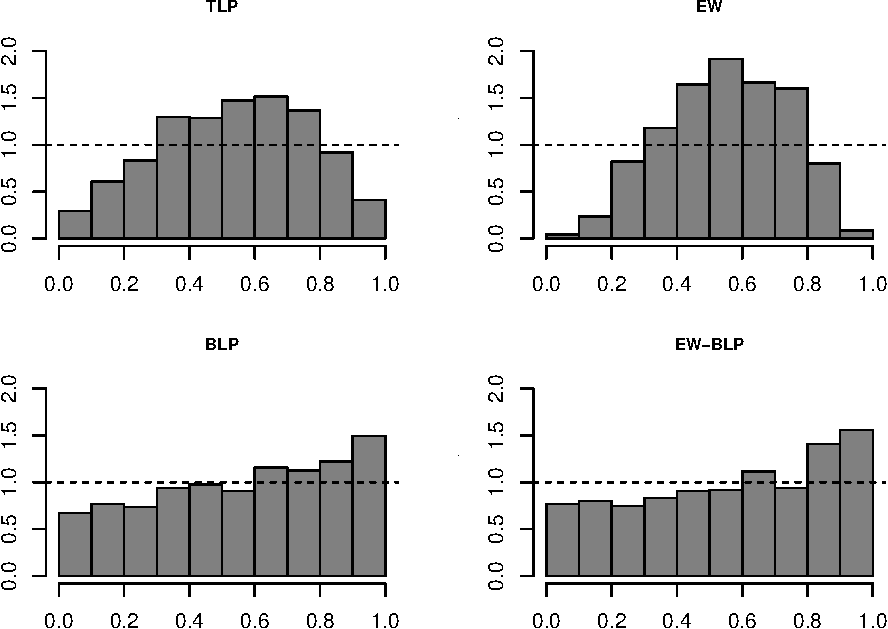
\includegraphics{BLPcalibration_app_files/figure-latex/unnamed-chunk-6-1.pdf}

\hypertarget{week-ahead---201718}{%
\subsubsection{1 week ahead - 2017/18}\label{week-ahead---201718}}

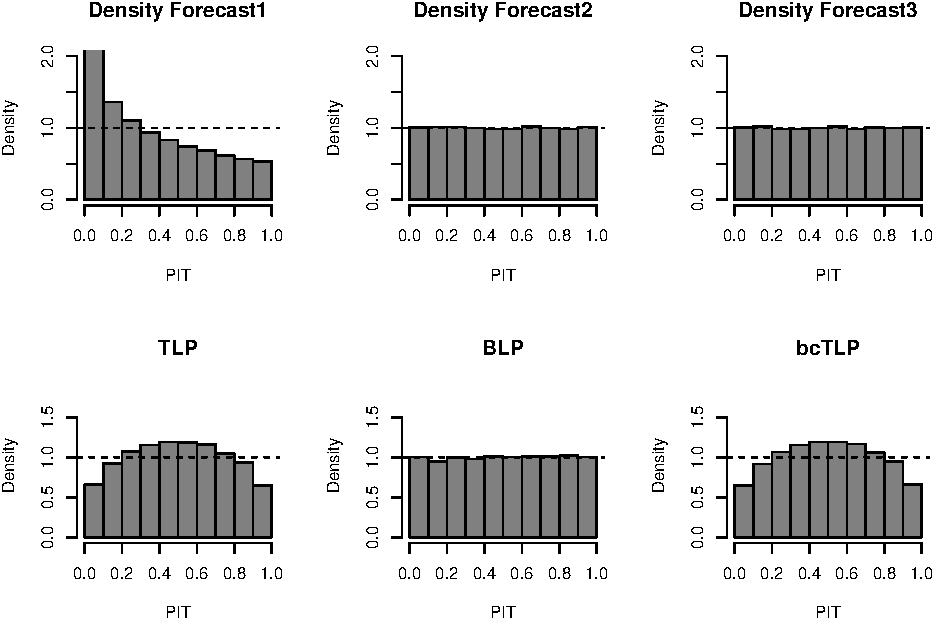
\includegraphics{BLPcalibration_app_files/figure-latex/unnamed-chunk-7-1.pdf}

\hypertarget{week-ahead---201617-1}{%
\subsubsection{2 week ahead - 2016/17}\label{week-ahead---201617-1}}

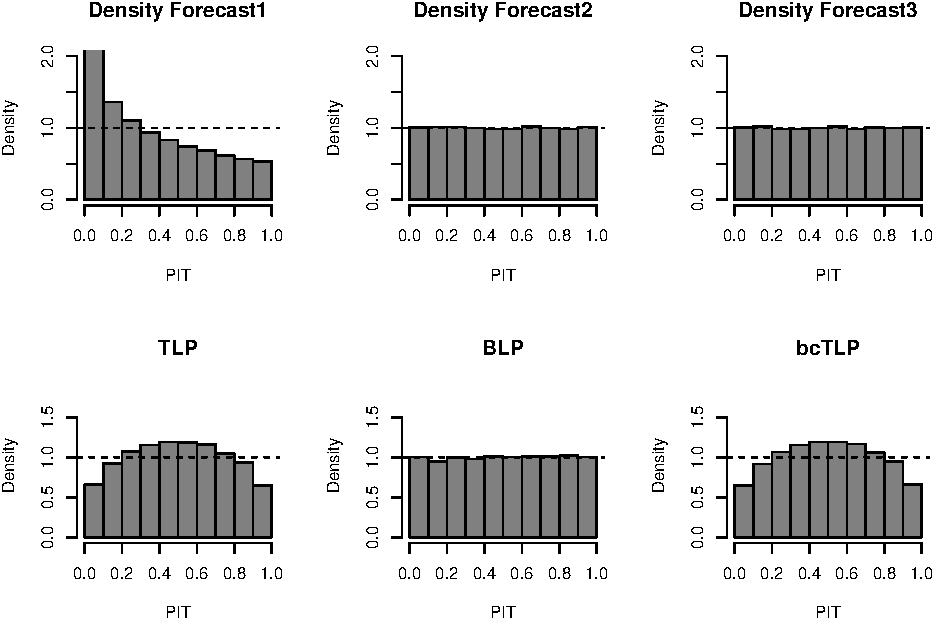
\includegraphics{BLPcalibration_app_files/figure-latex/unnamed-chunk-8-1.pdf}

\hypertarget{week-ahead---201718-1}{%
\subsubsection{2 week ahead - 2017/18}\label{week-ahead---201718-1}}

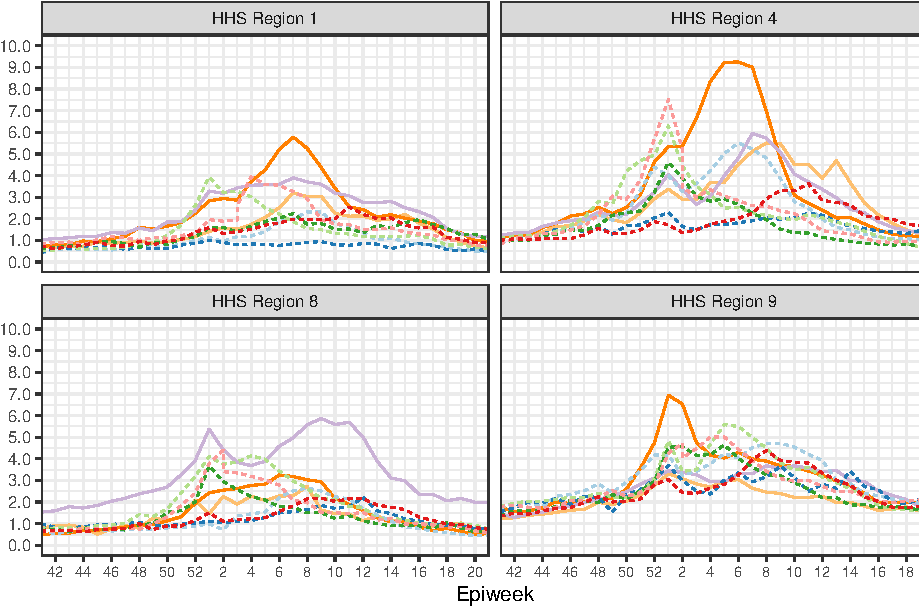
\includegraphics{BLPcalibration_app_files/figure-latex/unnamed-chunk-9-1.pdf}

\hypertarget{week-ahead---201617-2}{%
\subsubsection{3 week ahead - 2016/17}\label{week-ahead---201617-2}}

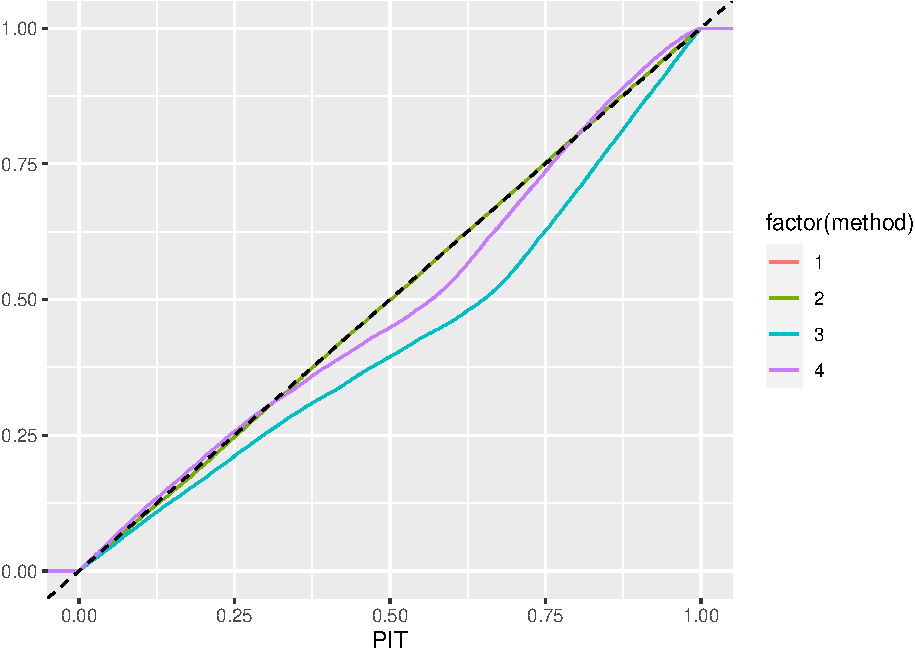
\includegraphics{BLPcalibration_app_files/figure-latex/unnamed-chunk-10-1.pdf}

\hypertarget{week-ahead---201718-2}{%
\subsubsection{3 week ahead - 2017/18}\label{week-ahead---201718-2}}

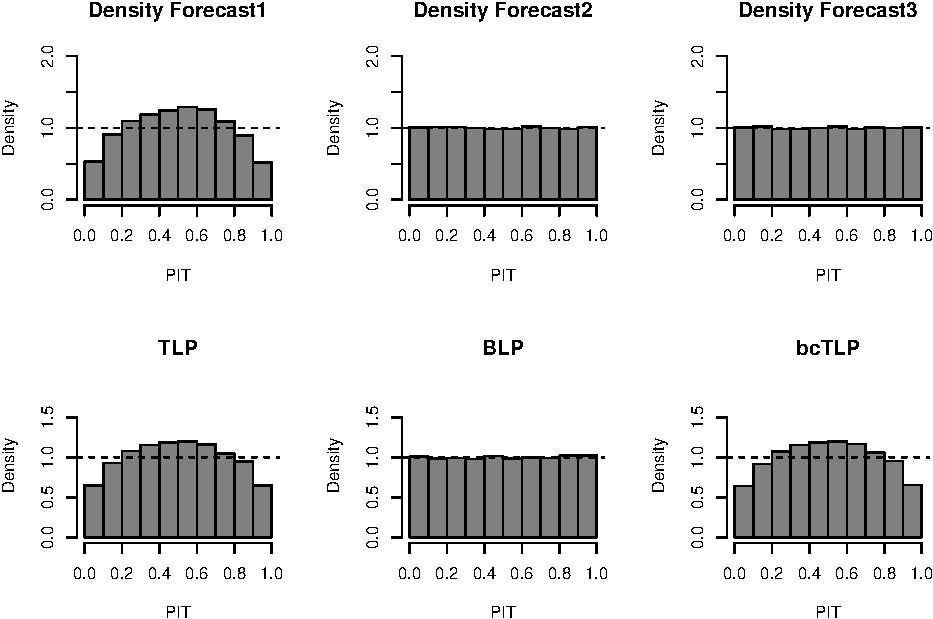
\includegraphics{BLPcalibration_app_files/figure-latex/unnamed-chunk-11-1.pdf}

\hypertarget{week-ahead---201617-3}{%
\subsubsection{4 week ahead - 2016/17}\label{week-ahead---201617-3}}

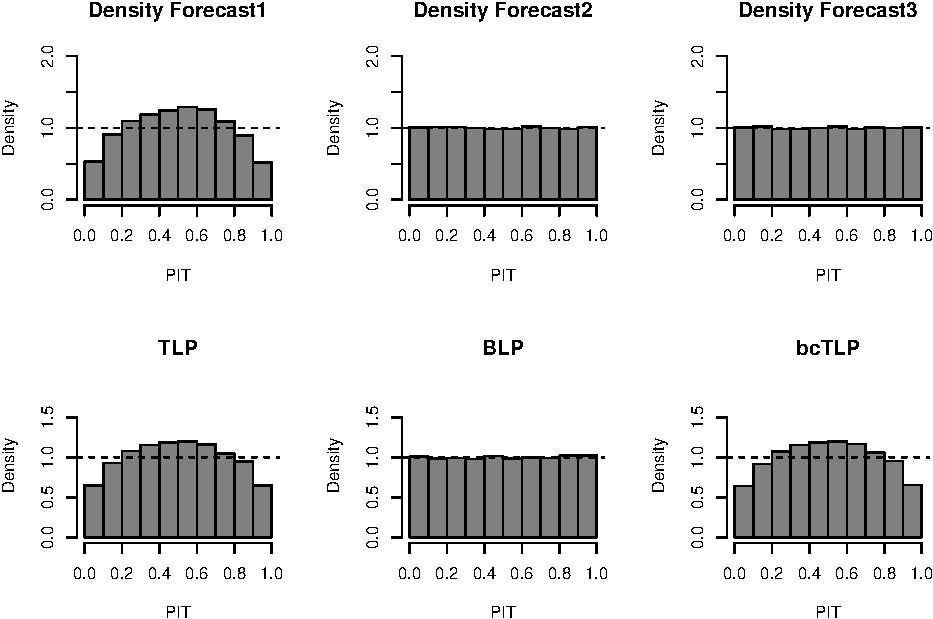
\includegraphics{BLPcalibration_app_files/figure-latex/unnamed-chunk-12-1.pdf}

\hypertarget{week-ahead---201718-3}{%
\subsubsection{4 week ahead - 2017/18}\label{week-ahead---201718-3}}

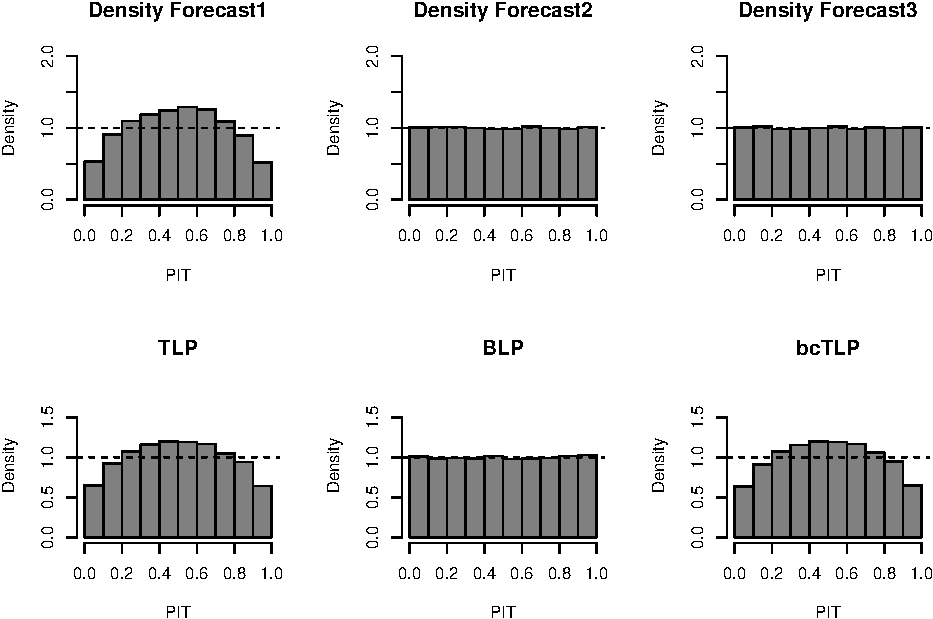
\includegraphics{BLPcalibration_app_files/figure-latex/unnamed-chunk-13-1.pdf}

\end{document}
